\chapter{Analýza a návrh řešení}
Tato kapitola se dělí na analýzu a návrh. V analýze jsem se zaměřil na prostudování tří existujících řešení. Z informací získaných z dokumentace jsem sestavil návrh pro Ruby ACL.

\section{Analýza}

Protože práce byla velmi přesně zadána, nezbylo příliš prostoru na různé alternativy. Ruby bylo zadáno jako implementační prostředí. Způsob zpracování byl zadán pomocí ACL. Hlavním úkol bylo zjistit, jakým způsobem implementovat samotné ACL a řádně implementaci zdokumentovat a otestovat.

\subsection{Exitující řešení}
\label{sec:anal-existujicireseni}

Při řešení vlastního návrhu na model řízení přístupových práv jsem vycházel ze dvou zdrojů – známých řešení a jednoho obecného řešení.

\subsubsection{Obecné řešení}
Obecným řešením je držet si tabulku, kde ve sloupcích budou objekty, ke kterým je možno přistupovat a v řádcích jsou přistupující. V poli pak jsou hodnoty boolean, které vyjadřují buď allow nebo deny. Příklad tabulkového řešení je v tabulce \ref{tab:tab2}.
\begin{table}%[h]
\centering
\begin{tabular}{|r||c|c|c|}
\hline
Kdo / Kam & Operační sál & Ambulance & Pokoj pacienta\\
\hline\hline
Chirurg & 1 & 1 & 1\\
\hline
Sestřička & X & 1 & 1\\
\hline
Pacient & X & X & 1\\
\hline
\end{tabular}
\caption{Jednoduchý příklad obecného řešení modelu práv pomocí matice}
\label{tab:tab2}
\end{table}

%-------------------------------------

\subsubsection{Oracle}
Jedním z řešení je firemní řešení prezentované v Oracle® XML DB Developer's Guide, 11g Release 1 (11.1), Part Number B28369-04 na stránkách Oracle dokumentace \cite{oracle}. Ve stati Access Control Lists and Security Classes je popsán koncept firmy ORACLE.
 
Text popisuje několik podmínek a pojetí řízení přístupu. Každá z popsaných entit, uživatel, role, privilegia, bezpečnostní třídy, Access Control List (ACL) a Access Control Entry (ACE), je realizována deklarativně jako XML dokument nebo fragment.  

Bezpečnostní autorizace vyžaduje definovat, kteří uživatelé, aplikace nebo funkce mohou mít přístup k jakým datům nebo jaké druhy operací mohou provádět. Existují tedy tři dimenze: (1) kteří uživatelé mohou, (2) vykonávat jaké činnosti, (3) na jakých datech. V souvislosti s každou jednotlivou dimenzí hovoříme o (1) principals - zmocnitelích, (2) privileges - oprávněných, a (3) objektech, které korespondují s těmito třemi dimenzemi. Principals mohou být uživatelé nebo role/skupiny.

Principals a privileges (dimenze 1 a 2) jsou deklarativním způsobem spojeni v definovaných seznamech řízení přístupu - ACL. Ty jsou pak spojené s třetí dimenzí - daty, různými způsoby. Například úložiště zdrojů nebo tabulky dat Oracle XML DB mohou být ochráněny pomocí PL / SQL procedury DBMS\_XDB.setACL nastavením jeho řídícího ACL.

%-------------------------------------

\subsubsection{phpGACL}
Druhým ze zdrojů, z nichž jsem vycházel, je řešení prezentované v Generic Access Control List with PHP - phpGACL na \cite{phpGACL}.

Nástroj phpGACL je sada funkcí, která umožňuje použít řízení přístupu na libovolné objekty (webové stránky, databáze, atd.), jiným libovolným objektům (uživatelé, vzdálené počítače, atd.). 
Stejně jako Oracle nabízí jemně nastavitelnou kontrolu přístupu s jednoduchou a velmi rychlou správou. Je napsán v populárním dynamickém skriptovacím jazyku PHP.

Nástroj phpGACL vyžaduje relační databáze pro ukládání informací k řízení přístupu. Přistupuje k databázi prostřednictvím tzv. abstraktního obalu ADOdb. Je kompatibilní s databázemi, jako PostgreSQL, MySQL a Oracle. 

Nástroj phpGACL používá pojmy jako ACO a ARO:
\begin{itemize}
\item Access Control Objects (ACO), jsou věci, ke kterým chceme ovládat přístup (např. webové stránky, databáze, pokoje, atd.).
\item Access Request Objects (ARO), jsou věci, které žádají o přístup (např. osoby, vzdálené počítače, atd.)
\item ARO stromy definují hierarchii skupin a ARO. Skupiny mohou obsahovat jiné skupiny a ARO.
\item Výchozí "catch-all" politikou stromu ARO je vždy "DENY ALL ".
\item Chceme-li přiřadit přístupovou politiku ve stromu směrem dolů, explicitně přiřazujeme oprávnění skupinám a ARO pro každou ACO, pro kterou je potřeba.
\end{itemize}

\section{Návrh implementace}
Při návrhu implementace jsem se inspiroval jak Oraclem tak phpGACL. Oba modely řízení přístupových práv mají podobnou strukturu nebo stejnou s jiným pojmenováním. Z Oraclu jsem převzal koncept a pojmenování dimenzí: principals, privileges, objects, ze kterých jsem vytvořil hlavní třídy. 

Jemně nastavitelných přístupových práv se docílí pomocí Access Control Listu. ACL obsahuje seznam pravidel jednotlivých přístupů. Pravidlo se nazývá Access Control Entry (ACE). V ACE je uloženo \textbf{kdo}, nebo \textbf{co} má jaká \textbf{práva} přistupovat k jakým \textbf{objektům}. Těmto třem rozměrům se v problematice přístupových práv říka: principals - zmocnitelé, privileges - oprávnění, resource objects - zdrojové objekty. Pokud mluvím o ACL objektu, myslím tím ACE nebo principal nebo privilege nebo resource object.

%---------------------------------------------------------------

\subsection{Use Case Scénáře}

%\begin{verbatim}\end{verbatim}
\subsubsection{Ověřování oprávnění k objektu}
Uživatel má vytvořenou instanci třídy RubyACL, která pracuje s již vytvořenými ACL objekty. Následující scénář popisuje jednotlivé kroky při kontrolování pravidla.

Hlavní úspěšný scénář:
\begin{enumerate}
\item Uživatel zavolá metodu \verb|check|. Přes tuto metodu se dotáže knihovny, jestli uživatel/skupina (ne)mají oprávnění ke zdrojovému objektu.
\item a) Systém vrátí true v případě, že uživatel/skupina má specifikované nebo vyšší oprávnění.
\item b) Systém vrátí false v případě, že uživatel/skupina nemají specifikované nebo vyšší oprávnění.
\end{enumerate}
Rozšíření:

0a) Pokud neexistuje žádné pravidlo, systém vrátí false, protože nenašel, žádné vyhovující pravidlo.
%\begin{verbatim}\end{verbatim}

%-----------------------------

\subsubsection{Zadávání pravidla (ACE)}
Uživatel má vytvořenou instanci RubyACL, která obsahuje pravidla.
Hlavní úspěšný scénář:
\begin{enumerate}
\item Uživatel zavolá metodu set\_new\_ace a specifikuje údaje (Uživatel/skupina, typ přístupy (allow/deny), oprávnění, zdrojový objekt
\item Knihovna nastaví pravidlo a vrátí 0, když vše proběhlo v pořádku, a 1 když nastala chyba.
\end{enumerate}
Poznámka: Jde vlastně o přiřazování oprávnění uživatelům na objekt

%---------------------------------------------------------------

\subsection{Rozhraní}
S knihovnou Ruby-ACL je zapotřebí komunikovat prostřednictvím rozhraní. Knihovna Ruby-ACL se nachází mezi databází, kde jsou uložené data o přístupech a uživatelskou aplikací, která knihovnu používá. Z tohoto důvodu jsem tuto sekci rozdělil na dvě podsekce. Jedna podsekce popisuje rozhraní mezi knihovnou a databází a druhá podsekce popisuje rozhraní mezi knihovnou a uživatelskou aplikací. 


\subsubsection{Rozhraní mezi Ruby-ACL a databází}
Rozhraní mezi Ruby-ACL a databází je zprostředkováno pomocí API\footnote[1]{Application Programming Interface}.
Ruby-ACL bylo testováno s databází eXist-db, se kterou komunikovalo pomocí mnou naimplemetovaného rozhraní eXistAPI. 
K používání Ruby-ACL s jinou XML databází než eXist-db je nutné komunikační rozhraní, které nahradí eXistAPI.
V ukázkové třídě API je výčet všech potřebných metod, které Ruby-ACL používá, včetně popisu parametrů a výstupů. Pro funkčnost knihovny s jinou XML databází je potřeba podle vzorové třídy API naimplementovat nové komunikační rozhraní. 
Podrobnější popis rozhraní se nachazí v příloženém CD jako prázdná třída zdokumentovaná pomocí RDOC\footnote[2]{Dokumentace pro zdrojové kódy v Ruby}. Na této části rozhraní záleží bezpočenost. Linka mezi API a databází je potencionálně nebezpečné místo k útoku.

\noindent Rozhraní mezi Ruby-ACL a databází zproztředkovává rozhraní API. To je patrné na obrázku diagramu komunikace \ref{fig:Communication diagram} v krocích 2 a 5.

\noindent Obrázek \ref{fig:API_interface} zobrazuje model tříd rozhraní API.

\begin{figure}
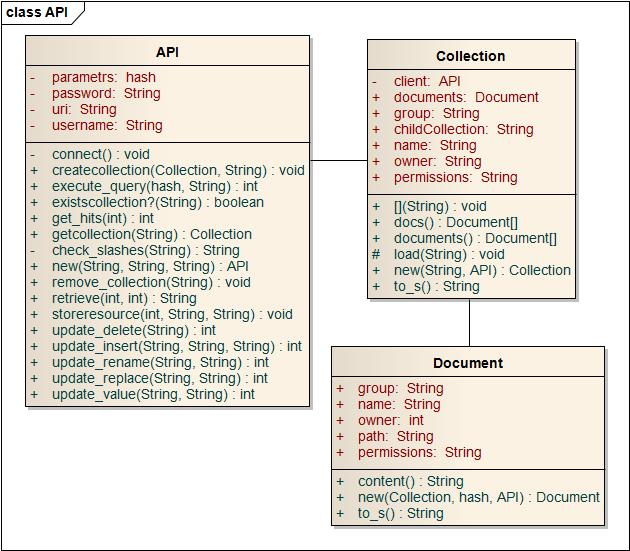
\includegraphics[width=15cm]{API1.jpg}
\caption{Diagram znázorňující model rozhraní}
\label{fig:API_interface}
\end{figure}

%----------------------------

\subsubsection{Rozhraní mezi Ruby-ACL a uživatelskou aplikací}
Rozhraní mezi knihovnou a uživatelskou aplikací tvoří všechny veřejné (public) metody třídy RubyACL. Pomocí instance této třídy a instance třídy API (která je předaná jako parametr) a následném volání veřejných metod může uživatel zavádět zmocnitele, oprávnění, zdrojové objekty a pravidla a pracovat s nimi.Výčet veřejných metod se nachází v příloze \ref{sec:veřejné metody}.

Nejčastěji používanou částí knihovny bude metoda \verb|check|. Mimo správu ACL objektů je hlavní účel knihovny rozlišit, jestli někdo nebo něco má oprávnění na nějaký zdrojový objekt. Pokud zmocnitel má nebo nemá přístup se uživatel dozví podle výstupu. Výstupem je true nebo false hodnota. Stručný popis nejčastějších vstupů a výstupů je v tabulce \ref{tab:tab3}

\begin{table}%[h]
\centering
\begin{tabular}{|c|c|c|}
\hline
\textbf{jméno} & \textbf{typ} & \textbf{popis}\\
\hline
\multicolumn{3}{|l|}{Vstupy} \\
\hline
principal & string & jméno zmocnitele\\
\hline
privilege & string & název oprávnění\\
\hline
resource object type & string & typ - druh zdrojového objektu\\
\hline
resource object address & string & adresa zdrojového objektu\\
\hline
\hline
\multicolumn{3}{|l|}{Výstupy} \\
\hline
access & boolean & true = přístup povolen, false = přístup zakázán\\
\hline
\end{tabular}
\caption{Parametry a návratové hodnoty metody check} %\verb|check|}
\label{tab:tab3}
\end{table}

%----------------------------------------------------

\subsection{Ukázka použití}
Tato sekce prezentuje stručné ale funkční ukázky použití.

%-----------------------------

\subsubsection{Příklad nastavení práv}
První příklad ukazuje, základní funkčnost knihovny a vytvoření pravidla. 
Protože knihovny Ruby-ACL vyžaduje jako jeden z parametrů instanci rozhraní API, bylo v příkladě použita implementace rozhraní eXistAPI. Pro vytvoření pravidla musí existovat instance Ruby-ACL. Ke správnému vytvoření pravidla musí být všechny ACL objekty vytvořené. Pokud nebudou vytvořené, Ruby-ACL vyhodí vyjímku, nebo ACL Objekt založí. Metodě \verb|create_ace| je potřeba předat uživatelské jméno zmocnitele, typ přístupu (allow nebo deny), oprávnění a požadovaný objekt identifikovaný pomocí typu objektu a adresy.

\begin{lstlisting}
require 'eXistAPI'    #must require 'eXistAPI' to comunicated with eXist-db
#creates instance of ExistAPI
@db = ExistAPI.new("http://localhost:8080/exist/xmlrpc", "admin", "password")    
@col_path = "/db/test_acl/"         #sets the collection where you want to have ACL in db
@src_files_path = "./src_files/"    #path to source files
@my_acl = RubyACL.new("my_acl", @db, @col_path, @src_files_path, true)
#it's good to create some principals at the begging
@my_acl.create_principal("Sheldon")
@my_acl.create_privilege("SIT")
@my_acl.create_resource_object("seat", "/livingroom/couch/Sheldon's_spot", "Sheldon")	#(type, address, owner) of resource object
@my_acl.create_ace("Sheldon", "allow", "SIT", "seat", "/livingroom/couch/Sheldon's_spot")	#(principal, acc.type, privilege, resOb type, adr)
\end{lstlisting}

%-----------------------------

\subsubsection{Příklad kontroly práv}
Následující příklad prezentuje možné použití knihovny a její metody \verb|check|. V případě, že metoda vratí hodnotu true, přístup povolen a aplikace provede co zamýšlela provést. Pokud vrátí hodnotu false, tak je přístup zamítnut. 

\begin{lstlisting}[firstnumber=12]
#Next method in if returns deny
if(@my_acl.check("Penny", "SIT", "seat", "/livingroom/couch/Sheldon's_spot"))
	puts "Access allowed. You may retrive resource object."
else
	puts "Access denied."
\end{lstlisting}

Co se děje při volání metody \verb|check| názorně vysvětluje obrázek \ref{fig:Communication diagram} zobrazující sekvenci komunikace. Kroky 7 a vyšší jsou volitelné v případě, že je přístup povolen.
\begin{enumerate}
\item Výkonná část uživatelské aplikace zavolá metodu \verb|check| třídy RubyACL
\item Metoda \verb|check| vytvoří xQuery dotaz a předá ho implementaci rozhraní API zavoláním metody \verb|execute_query|
\item API se pomocí XML-RPC protokolu dotáže databáze
\item databáze vrátí výsledek(y)
\item API předá výsledk(y) metodě \verb|check|
\item Metoda \verb|check| z výsledků rozhodne, jestli principal má oprávnění na zdrojový objekt a podle toho vrátí boolean hodnotu; Více o priority rozhodování se lze dočíst TODO

---------

\item Uživatelská aplikace zavolá \verb|execute_query|
\item \verb|execute_query| pomocí XML-RPC zažádá o objekt
\item databáze vrátí objekt
\item \verb|execute_query| předá objekt uživatelské aplikaci
\end{enumerate}

\begin{figure}
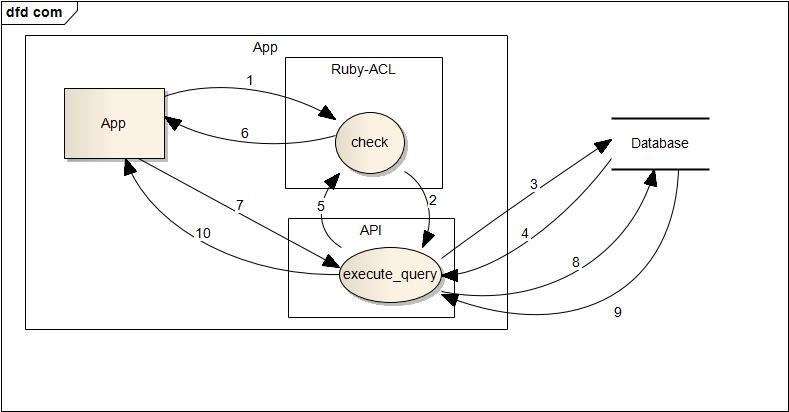
\includegraphics[width=15cm]{com.jpg}
\caption{Diagram znázorňující sekvenci komunikace}
\label{fig:Communication diagram}
\end{figure}



%---------------------------------------------------------

\subsection{Class diagram}
Class diagram \ref{fig:Class diagram} znázorňuje třídy knihovny a jejich vazby. Diagram je zjednodušen - nejsou vypsány všechny metody a paramatery z důvodů přehlednosti a čitelnosti. 

Hlavní třídou knihovny je třída RubyACL. Pomocí ní a jejích veřejných metody pracuje uživatelská aplikace s ACL objekty. Třída RubyACL obsahuje jen jednu instanci od každé třídy dědící z ACL\_Object. Tyto třídy jsou pomocné třídy, které "znají" strukturu dokumentu uloženého v databázi. Například s pomocí instance třídy ACE lze přidávat, měnit a mazat jednotlivé pravidla, které jsou v databázi v XML souboru reprezentovány jako uzly. Více o struktuře XML souborů se lze dočíst v TODO

Druhou podstatnou třídou je třída ACL\_Object, ze které dědí všechny pomocné třídy. Třídu ACL\_Object jsem vytvořil, protože velká část kód tříd Principal, Privilege, ResourceObject, ACE, Group, Individual se schodovala nebo byla velmi podobná. Vyjmenované podtřídy využívají zděděné metody a případně je konkrétizují.
Třída ACL\_Object obsahuje metody, které pomocí xQuery a xPath obsluhují rozhraní API, v tomto případě eXistAPI.

Z diagramu je patrné, že všechny data jsou uložené v databázi ve formě XML dokumentů, kde se na ně dotazuje rozhraní API.

\begin{figure}
%\centering
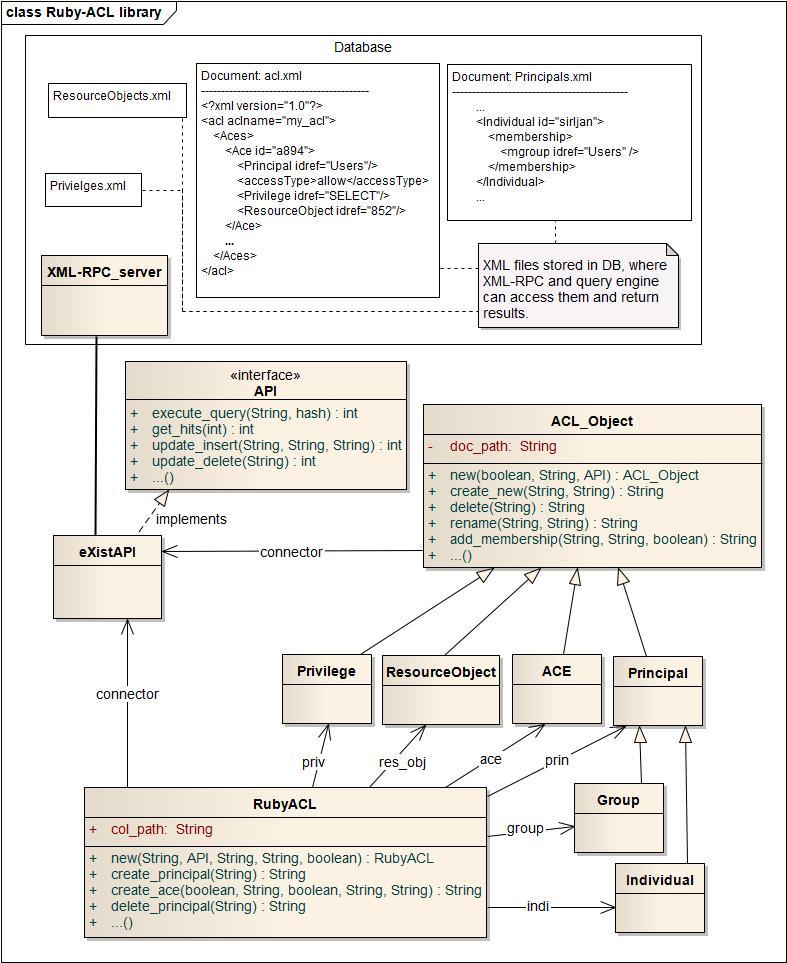
\includegraphics[width=15cm]{Ruby-ACL.jpg}
\caption{Class diagram}
\label{fig:Class diagram}
\end{figure}

%-------------------------------------
\section{Popis logiky vyhodnocování pravidel}
V této kapitole je popsáno jakým způsobem Ruby-ACL rozhoduje, jestli je přístup povolen či nikoliv. Nejkonkrétněji se tímto zabývá sekce "Pravidla rozhodování", nicméně k pochopení celku je dobré vědět vlastnosti jednotlivých ACL objektů. O nich se dočtete ve sekci ACL\_Objekty.

\subsection{ACL Objekty}
Jak již bylo v předchozí části textu řečeno. ACL objekt je principal, privilege, resource object, ACE. Principal se dále dělí na individual a group. Data, která jsou uložena v databázi ve formě XML dokumentů, jsou vlastně všechny ACL objekty. Každý ACL objekt má dedikovaný soubor vyjma individual a group. Tyto ACL objekty se ukládají do Principals.xml, protože jsou podmnožinou principal.

Ruby-ACL pracuje s daty tak, že za pomoci jedné ze tříd, které dědí ze třídy ACL\_Object, edituje XML soubory v databázi. Upravuje je takovým způsobem, že přidává, maže nebo mění jednotlivé uzly.

Struktura XML souboru je popsaná pomocí DTD\footnote[1]{Document Type Definition} souboru v příloze na CD. Pro každý ACL objekt, ale vyjadřuji v příslušné sekci i slovně.

\subsubsection {Zmocnitel (Principal)}
Principal nebo-li zmocnitel může být jednotlivec nebo skupina. Jednotlivec může být člověk jako uživatel nebo proces, aplikace, připojení, zkrátka cokoliv, co vyžaduje přístup.

Skupiny a jednotlivci se ukládají do souboru Principals.xml.
Vyjádření strukturu slovy, je následující. Principals.xml obsahuje kořenový uzel Principals ten obsahuje pouze dva uzly Groups a Individuals. V uzlu Groups může byt neomezené množství uzlů Group, které reprezentují skupiny. V uzlu Individuals může být neomezené množství uzlů Individual. 

Jednotlivci a skupiny se můžou sdružovat do skupin. Každý jednotlivec nebo skupina má v sobě v uzlu membership odkaz(y) v jaké skupině je členem. To obstarává uzel mgroup s atributem idref na danou skupinu. Nelze, aby jednotlivec byl členem v jednotlivcovi.

\lstset{language=XML}
\begin{lstlisting}
<Principals>
    <Groups>
        <Group id="ALL">
            <membership/>
        </Group>
        <Group id="Users">
            <membership>
                <mgroup idref="ALL"/>
            </membership>
        </Group>
    </Groups>
    <Individuals>
        <Individual id="sirljan">
            <membership>
                <mgroup idref="Users" />
                <mgroup idref="Developers" />
            </membership>
        </Individual>
    </Individuals>
</Principals>
\end{lstlisting}

\subsubsection {Oprávnění (Privilege)}
Ruby-ACL nabízí výchozí oprávnění, které jsem převzal od Oracle a MySQL. To jestli je uživatel použije, záleží na něm. 
Výchozí privilegia jsou: 'ALL PRIVILEGES', 'ALTER', 'CREATE', 'DELETE', 'DROP', 'FILE', 'INDEX', 'INSERT', 'PROCESS', 'REFERENCES', 'RELOAD', 'SELECT', 'SHUTDOWN', 'UPDATE' a 'USAGE'.
Pravidla lze vytvářet a seskupovat do stromové struktury.

Oprávnění se ukládají do souboru Privileges.xml. Ten obsahuje kořenový uzel Privileges, ve kterém je neomezené množství uzlů Privilege. Stejně jako Individual nebo Group, Privilege obsahuje uzel membership a v něm neomezené množství uzlů mgroup, které pomocí idref odkazují na nadřazené oprávnění.

\begin{lstlisting}
<Privileges>
    <Privilege id="SELECT">
        <membership>             
            <mgroup idref="ALL_PRIVILEGES" />         
        </membership>
    </Privilege>
</Privileges>
\end{lstlisting}

\subsubsection {Zdrojový objekt (Resource object)}

Zdrojové objekty jsou ukládány do souboru ResourceObjects.xml. Struktura je opět podobná předchozím ukázkám. Kořenový uzel je ResourceObjects a v něm je neomezené množství uzlů ResourceObject.

\begin{lstlisting}
<ResourceObjects>
    <ResourceObject id="r753951654">
        <type>doc</type>
        <address>/db/cities/cities.xml/cities</address>
        <owner idref="sirljan"/>
    </ResourceObject>
\end{lstlisting}


Skládá se ze tří položek: typ, adresa, vlastník. Typ může být dokument, nebo reálné objekty jako dveře, místnosti apod. Adresa společně s type identifikuje objekt. Zdrojový objekt jasně identifikuje i id v parametru každého ResourceObject uzlu, ale uživatel velmi pravděpodobně nebude vědět id zdrojových objektů. Uživatel by sice mohl id zjistit pomocí metody \verb|find_res_ob| třídy ResourceObject, ale stejně by musel zadat typ a adresu. Vlastník objektu může být jakýkoliv principal.


TODO co se stane kdyz se zalozi objekt doc("/db/cities/cities.xml")/cities
TODO se typ nenachazi v adresse

Při zadávání adresy je potřeba dodržet jediné pravidlo. V adrese oddělovat každý jednotlivý objekt dopředným lomítkem. ( / )

Pokud je zdrojový objekt typu doc, adresa může obsahovat klauzuli ve formátu ("/koren/vetev/list-soubor\_s\_příponou") a pokud je zapotřebí jemnější řízení přístupu uvnitř dokumentu následuje klauzule /koren/vetev. Nicméně do databáze se ukládá sloučená adresa bez ("")
Příklad:  ("/db/data/cities.xml")/cities/city
V databázi je uložen pod adresou: /db/data/cities.xml/cities/city
Tento způsob byl zvolen kvůli jednoduším rozhodování a parsování.

Klauzule /* (lomítko hvězdička) vyjadřuje všechny podřadné objekty
Příklad:  /db/data/*
Nyní jsou vybrány všechny podřadné objekty objektu data.
/* nemá význam u vlastníka, protože vlastník zdrojového objektu vlastní i všechny podřazené zdrojové objekty.

Vlastník / Owner
Owner může být jednotlivec, množina jednotlivců i skupina.
Množina jednotlivců je v případě pokud se od kořene zdrojových objektů k listu mnění vlastník. Vlastník nejnadřazenějšího zdroje má největší práva. Vlastník může být o 
/* nemá význam, protože vlastník zdrojového objektu vlastní i všechny podřazené zdrojové objekty.

\subsubsection{Pravidlo (ACE)}

Pokud přijde žádost o vytvoření ACE s neexistujícím zdrojovým objektem, knihovna objekt vytvoří. Z toho vyplývá, že v databázi existují všechny zdrojové objekty sjednocené s objekty, které byli vytvořeny přímo.

\begin{verbatim}
        <Ace id="a894">
            <Principal idref="Users"/>
            <accessType>allow</accessType>
            <Privilege idref="SELECT"/>
            <ResourceObject idref="852"/>
        </Ace>
\end{verbatim}

\subsection{Složitost rozhodování}
Slozitost je e\^2.

%--------------------------------

\subsection{Pravidla rozhodování}
\subsubsection{Priorita rozhodování}

Nejnižší má největší prioritu.

\begin{enumerate}
\item Owner
\item Explicit Deny
\item Explicit Allow
\item Inherited Deny
\item Inherited Allow
\item If not found > Deny
\end{enumerate}
